\ylDisplay{Magnetväli} % Ülesande nimi
{Jaan Kalda} % Autor
{piirkonnavoor} % Voor
{2010} % Aasta
{G 9} % Ülesande nr.
{9} % Raskustase
{
% Teema: Magnetism
\ifStatement
Magnetväli induktsiooniga $B$ täidab joonisel kujutatud mõõtmetega risttahukakujulist ruumipiirkonda, välja arvatud väga kitsas magnetväljata pilus.
Joonisel näidatud suunas lendab kiirusega $v$ elektron (massiga $m$ ja laenguga $e$). Arvutage ja visandage graafikul, kuidas sõltub elektroni kõrvalekaldenurk (st nurk tema kiirusvektorite vahel enne magnetvälja sisenemist ja peale sealt lõplikku väljumist) elektroni algkiirusest $v$; piirduge väärtustega $v<2aBe/m$.
\begin{center}
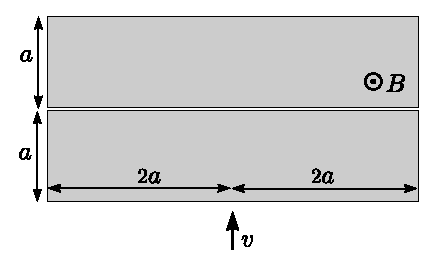
\includegraphics[width=0.5\linewidth]{2010-v2g-09-elektron.eps}
\end{center}
\fi


\ifHint
Magnetväljas hakkab osake liikuma mööda ringjoont. Ringjoone raadius on avaldatav Lorentzi jõu ja kesktõmbekiiruse võrdsusest.
Märkame, et kui ringjoone raadius on piisavalt väike, väljub elektron tuldud suunas tagasi. Ringjoone suurenedes väljub elektron lõpuks vasakust küljest.
\fi


\ifSolution
Magnetväljas mõjub elektronile Lorentzi jõud $F=Bev$, mis on kiirusega kogu aeg risti ning
annab elektronile kesktõmbekiirenduse $v^2/R$, kus $R$ on trajektoori kõverusraadius. Newtoni teisest seadusest $Bev=mv^2/R$, millest $R=vm/Be$.

Et elektroni kiirus ei muutu (energia säilib!), siis ka kõverusraadius ei muutu, st elektron liigub mööda ringjoont raadiusega $R$.
Tuues sisse tähistuse $v_0=aBe/m$, saame eelmise avaldise kirjutada kujul $R=vm/Be=va/v_0$.

Kui $v< v_0$, siis elektron teeb magnetväljas poolringi ning väljub tuldud suunas tagasi,
st pöördenurk on $\SI{\pi}{rad}$. Vastva graafikuosa eest.

Kui $v\approx v_0$, siis saab elektron väljuda mööda kitsast pilu, vt joonist, st pöördenurk on $\SI{\pi/2}{rad}$. Vastva graafikuosa eest.

\begin{center}
	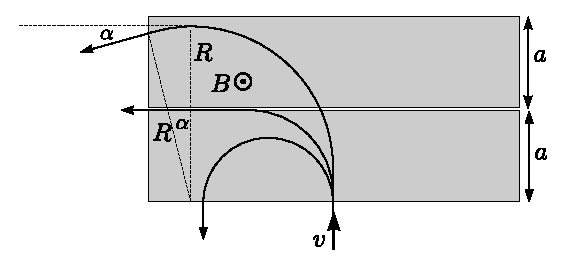
\includegraphics[width=0.6\textwidth]{2010-v2g-09-elektronlah.eps}
\end{center}

Kiiruse edasisel suurenemisel väljub elektron külgsuunas; joonise abil on lihtne näha, et väljumisnurk on
\[
\alpha =\frac \pi 2 + \arcsin \frac{2a -R}{R}=\frac \pi 2 + \arcsin \left(2\frac {v_0}v -1\right).
\]
Kvalitatiivselt mõistliku graafikuosa eest, st graafikuosa algab väärtuselt $\SI{\pi}{rad}$
ja lõppeb väärtuse $\SI{\pi/2}{rad}$ juures.

Kokkuvõtvalt on sõltuvus $\alpha (v)$ esitatud järgmisel leheküljel oleval graafikul.

\begin{center}
	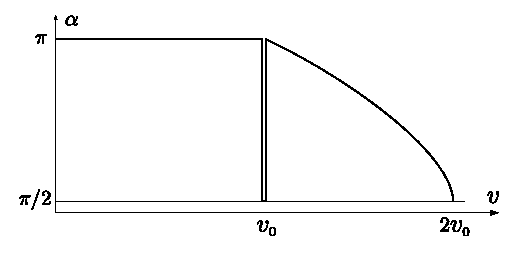
\includegraphics[width=0.6\textwidth]{2010-v2g-09-elektronlah2.eps}
\end{center}
\fi
}